% Options for packages loaded elsewhere
\PassOptionsToPackage{unicode}{hyperref}
\PassOptionsToPackage{hyphens}{url}
\PassOptionsToPackage{dvipsnames,svgnames,x11names}{xcolor}
\PassOptionsToPackage{space}{xeCJK}
%
\documentclass[
  11pt,
]{article}
\usepackage{amsmath,amssymb}
\usepackage{iftex}
\ifPDFTeX
  \usepackage[T1]{fontenc}
  \usepackage[utf8]{inputenc}
  \usepackage{textcomp} % provide euro and other symbols
\else % if luatex or xetex
  \usepackage{unicode-math} % this also loads fontspec
  \defaultfontfeatures{Scale=MatchLowercase}
  \defaultfontfeatures[\rmfamily]{Ligatures=TeX,Scale=1}
\fi
\usepackage{lmodern}
\ifPDFTeX\else
  % xetex/luatex font selection
  
  
\fi
% Use upquote if available, for straight quotes in verbatim environments
\IfFileExists{upquote.sty}{\usepackage{upquote}}{}
\IfFileExists{microtype.sty}{% use microtype if available
  
   % disable protrusion for tt fonts
}{}
\makeatletter
\@ifundefined{KOMAClassName}{% if non-KOMA class
  \IfFileExists{parskip.sty}{%
    \usepackage{parskip}
  }{% else
    \setlength{\parindent}{0pt}
    \setlength{\parskip}{6pt plus 2pt minus 1pt}}
}{% if KOMA class
  \KOMAoptions{parskip=half}}
\makeatother
\usepackage{xcolor}
\usepackage[margin=1in]{geometry}
\usepackage{color}
\usepackage{fancyvrb}
\newcommand{\VerbBar}{|}
\newcommand{\VERB}{\Verb[commandchars=\\\{\}]}
\DefineVerbatimEnvironment{Highlighting}{Verbatim}{commandchars=\\\{\}}
% Add ',fontsize=\small' for more characters per line
\newenvironment{Shaded}{}{}
\newcommand{\AlertTok}[1]{\textcolor[rgb]{1.00,0.00,0.00}{\textbf{#1}}}
\newcommand{\AnnotationTok}[1]{\textcolor[rgb]{0.38,0.63,0.69}{\textbf{\textit{#1}}}}
\newcommand{\AttributeTok}[1]{\textcolor[rgb]{0.49,0.56,0.16}{#1}}
\newcommand{\BaseNTok}[1]{\textcolor[rgb]{0.25,0.63,0.44}{#1}}
\newcommand{\BuiltInTok}[1]{\textcolor[rgb]{0.00,0.50,0.00}{#1}}
\newcommand{\CharTok}[1]{\textcolor[rgb]{0.25,0.44,0.63}{#1}}
\newcommand{\CommentTok}[1]{\textcolor[rgb]{0.38,0.63,0.69}{\textit{#1}}}
\newcommand{\CommentVarTok}[1]{\textcolor[rgb]{0.38,0.63,0.69}{\textbf{\textit{#1}}}}
\newcommand{\ConstantTok}[1]{\textcolor[rgb]{0.53,0.00,0.00}{#1}}
\newcommand{\ControlFlowTok}[1]{\textcolor[rgb]{0.00,0.44,0.13}{\textbf{#1}}}
\newcommand{\DataTypeTok}[1]{\textcolor[rgb]{0.56,0.13,0.00}{#1}}
\newcommand{\DecValTok}[1]{\textcolor[rgb]{0.25,0.63,0.44}{#1}}
\newcommand{\DocumentationTok}[1]{\textcolor[rgb]{0.73,0.13,0.13}{\textit{#1}}}
\newcommand{\ErrorTok}[1]{\textcolor[rgb]{1.00,0.00,0.00}{\textbf{#1}}}
\newcommand{\ExtensionTok}[1]{#1}
\newcommand{\FloatTok}[1]{\textcolor[rgb]{0.25,0.63,0.44}{#1}}
\newcommand{\FunctionTok}[1]{\textcolor[rgb]{0.02,0.16,0.49}{#1}}
\newcommand{\ImportTok}[1]{\textcolor[rgb]{0.00,0.50,0.00}{\textbf{#1}}}
\newcommand{\InformationTok}[1]{\textcolor[rgb]{0.38,0.63,0.69}{\textbf{\textit{#1}}}}
\newcommand{\KeywordTok}[1]{\textcolor[rgb]{0.00,0.44,0.13}{\textbf{#1}}}
\newcommand{\NormalTok}[1]{#1}
\newcommand{\OperatorTok}[1]{\textcolor[rgb]{0.40,0.40,0.40}{#1}}
\newcommand{\OtherTok}[1]{\textcolor[rgb]{0.00,0.44,0.13}{#1}}
\newcommand{\PreprocessorTok}[1]{\textcolor[rgb]{0.74,0.48,0.00}{#1}}
\newcommand{\RegionMarkerTok}[1]{#1}
\newcommand{\SpecialCharTok}[1]{\textcolor[rgb]{0.25,0.44,0.63}{#1}}
\newcommand{\SpecialStringTok}[1]{\textcolor[rgb]{0.73,0.40,0.53}{#1}}
\newcommand{\StringTok}[1]{\textcolor[rgb]{0.25,0.44,0.63}{#1}}
\newcommand{\VariableTok}[1]{\textcolor[rgb]{0.10,0.09,0.49}{#1}}
\newcommand{\VerbatimStringTok}[1]{\textcolor[rgb]{0.25,0.44,0.63}{#1}}
\newcommand{\WarningTok}[1]{\textcolor[rgb]{0.38,0.63,0.69}{\textbf{\textit{#1}}}}
\usepackage{longtable,booktabs,array}
\usepackage{calc} % for calculating minipage widths
% Correct order of tables after \paragraph or \subparagraph
\usepackage{etoolbox}
\makeatletter
\patchcmd\longtable{\par}{\if@noskipsec\mbox{}\fi\par}{}{}
\makeatother
% Allow footnotes in longtable head/foot
\IfFileExists{footnotehyper.sty}{\usepackage{footnotehyper}}{\usepackage{footnote}}
\makesavenoteenv{longtable}
\usepackage{graphicx}
\makeatletter
\def\maxwidth{\ifdim\Gin@nat@width>\linewidth\linewidth\else\Gin@nat@width\fi}
\def\maxheight{\ifdim\Gin@nat@height>\textheight\textheight\else\Gin@nat@height\fi}
\makeatother
% Scale images if necessary, so that they will not overflow the page
% margins by default, and it is still possible to overwrite the defaults
% using explicit options in \includegraphics[width, height, ...]{}
\setkeys{Gin}{width=\maxwidth,height=\maxheight,keepaspectratio}
% Set default figure placement to htbp
\makeatletter
\def\fps@figure{htbp}
\makeatother
\setlength{\emergencystretch}{3em} % prevent overfull lines
\providecommand{\tightlist}{%
  \setlength{\itemsep}{0pt}\setlength{\parskip}{0pt}}
\setcounter{secnumdepth}{-\maxdimen} % remove section numbering

% get rid of language-specific shorthands (see #6817):


\ifLuaTeX
  \usepackage{selnolig}  % disable illegal ligatures
\fi
\IfFileExists{bookmark.sty}{\usepackage{bookmark}}{\usepackage{hyperref}}
\IfFileExists{xurl.sty}{\usepackage{xurl}}{} % add URL line breaks if available
\urlstyle{same}
\hypersetup{
  pdftitle={Beyond the Slack Barrier: Lean-Verified Bounds and Counterexamples for Erd\texorpdfstring{\odoubleacute}{o}s 488},
  pdflang={en},
  colorlinks=true,
  linkcolor={Maroon},
  filecolor={Maroon},
  citecolor={Blue},
  urlcolor={Blue},
  pdfcreator={LaTeX via pandoc}}

\title{Beyond the Slack Barrier: Lean-Verified Bounds and
Counterexamples for Erd\texorpdfstring{\odoubleacute}{o}s 488}
\author{}
\date{5 September 2026}

\setmainfont[Path=fonts/,BoldFont=NotoSansCJKsc-Regular.otf,BoldFeatures={FakeBold=2},ItalicFont=NotoSansCJKsc-Regular.otf,ItalicFeatures={FakeSlant=0.15}]{NotoSansCJKsc-Regular.otf}
\XeTeXlinebreaklocale "zh"
\XeTeXlinebreakskip=0pt plus 1pt

\newfontfamily\accentfont[BoldFont=lmroman10-bold.otf,ItalicFont=lmroman10-italic.otf,BoldItalicFont=lmroman10-bolditalic.otf]{lmroman10-regular.otf}
\newcommand{\odoubleacute}{{\accentfont\char"0151}}

\begin{document}
\maketitle

\textbf{Research manuscript.} Project curator: \texttt{shoal-rat}.
Prepared through an AI-assisted research workflow using OpenAI Codex.
The curator handle is not an inferred human author name or affiliation;
no peer-review status is asserted. The accompanying Lean sources, rather
than this narrative, specify the certified statements exactly.

\hypertarget{abstract}{%
\subsection{Abstract}\label{abstract}}

For a finite primitive set of integers \(G\subseteq\mathbb N_{\ge2}\),
let \(F_G(n)\) count the positive integers at most \(n\) divisible by an
element of \(G\), and put \(I_G(n)=\sum_{g\in G}\lfloor n/g\rfloor\). We
give Lean-verified results concerning the density-doubling inequality in
Erd\texorpdfstring{\odoubleacute}{o}s problem 488. First, the auxiliary estimate
\(I_G(n)+|G|\le2F_G(n)\) holds whenever \(n\ge\max G\) and the excess
\(E=F_G(n)-|G|\) is at most 15. Consequently, the original strict
inequality holds at every such lower endpoint and every later upper
endpoint. A primitive, collectively coprime example with \(E=16\) shows
that 16 is the exact first failure of this auxiliary estimate. This
threshold persists at arbitrarily small covered density and arbitrarily
large lower endpoints, although the entire resulting sharp family still
satisfies the original inequality. We also give explicit counterexamples
to Conjectures 4.8 and 6.11 of a specified March 2026 manuscript, prove
unbounded tail-sifted density ratios for every fixed primitive ordered
pair, and prove unbounded incidence-to-coverage ratios under
simultaneous primitivity, collective coprimality, and arbitrary
sparsity. The finite classifications are checked by Lean's kernel, with
explicit completeness arguments and unchanged state transitions. The
unrestricted Erd\texorpdfstring{\odoubleacute}{o}s problem remains unresolved in this manuscript; global
priority for the strengthened formulations is not claimed.

\textbf{Keywords:} sets of multiples; primitive sets; density doubling;
finite certificates; Lean; computer-assisted mathematics.

\hypertarget{problem-notation-and-scope}{%
\subsection{1. Problem, notation, and
scope}\label{problem-notation-and-scope}}

Write \(\mathbb N=\{0,1,2,\ldots\}\). For a finite set
\(G\subseteq\mathbb N_{\ge2}\), define

\[
B_G=\{x\in\mathbb N:x\ge1,\ \exists g\in G, g\mid x\},\qquad
F_G(n)=|B_G\cap[1,n]|,
\] \[
I_G(n)=\sum_{g\in G}\left\lfloor\frac ng\right\rfloor.
\]

The formulation of Erd\texorpdfstring{\odoubleacute}{o}s problem 488 considered here asks whether every
nonempty finite \(A\subseteq\mathbb N_{\ge2}\) satisfies

\[
\boxed{\quad nF_A(m)<2mF_A(n)\qquad(m>n\ge\max A).\quad} \tag{1}
\]

This is the sets-of-multiples formulation in the archived formal
statement {[}1{]}. A set is \textbf{primitive} if \(a,b\in G\) and
\(a\mid b\) imply \(a=b\). Deleting elements divisible by other elements
leaves the same set of multiples and produces a primitive set. Thus
primitive sets are a natural setting for the argument.

Assume \(n\ge\max G\). Every generator is itself covered, so

\[
E_G(n):=F_G(n)-|G|\ge0.
\]

We call \(E_G(n)\) the \textbf{excess}. It counts covered points other
than generators. This is distinct from the signed slack
\(2F_G(n)-I_G(n)-|G|\). We use \textbf{collectively coprime} to mean
\(\gcd\{g:g\in G\}=1\), not that every pair of generators is coprime.

The arguments below address two different questions: how far a
particular auxiliary estimate proves (1), and why proposed auxiliary
assertions can fail without refuting (1). All unbounded statements
retain their displayed quantifiers. In particular, an unbounded family
of tail-sifted ratios is not a claim about a single fixed tail.

\hypertarget{main-results}{%
\subsection{2. Main results}\label{main-results}}

\textbf{Theorem 1 (the complete excess-at-most-fifteen bound).} Let
\(G\subseteq\mathbb N_{\ge2}\) be finite and primitive, and let
\(n\ge\max G\). If \(E_G(n)\le15\), then

\[
I_G(n)+|G|\le2F_G(n). \tag{2}
\]

If \(G\ne\varnothing\), then (1) holds for every integer \(m>n\).

The inequality (2) also holds for the empty set; only the strict
conclusion requires nonemptiness. For arbitrary nonempty finite
\(A\subseteq\mathbb N_{\ge2}\), let \(G\) be its divisibility-minimal
subset. The same conclusion holds under \(F_A(n)-|G|\le15\). Replacing
\(|G|\) here by the original \(|A|\) is not justified.

\textbf{Theorem 2 (a sharp auxiliary threshold, even under sparsity).}
Among primitive finite \(G\subseteq\mathbb N_{\ge2}\), with
\(n\ge\max G\), the smallest excess at which (2) fails is 16. More
strongly, for every \(R,M\in\mathbb N\), there are nonempty \(G\) and
\(n\) satisfying these conditions and

\[
\gcd(G)=1,\quad RF_G(n)<n,\quad 2F_G(n)<n,\quad M<n,
\] \[
E_G(n)=16,\qquad I_G(n)+|G|=2F_G(n)+1. \tag{3}
\]

For each prescribed \(R,M\), 16 remains the least failure excess under
all these restrictions. The construction used for (3) nevertheless
satisfies the original inequality at its specified lower endpoint for
\textbf{every positive} upper endpoint, in particular for every \(m>n\).

\textbf{Theorem 3 (unbounded density ratios after a finite prime tail).}
Fix integers \(2\le a<b\) with \(a\nmid b\). Define

\[
S_{a,b\mid V}(x)=\#\{1\le u\le x:(a\mid u\ \text{or}\ b\mid u),\
\forall p\in V, p\nmid u\}.
\]

For every \(K,M\in\mathbb N\), \(K\ge1\), there are a nonempty finite
set of primes \(V\subseteq\{p:p>b\}\) and integers \(n,m\) such that

\[
m>n> M,\qquad n\ge\max(V\cup\{a,b\}),\qquad S_{a,b\mid V}(n)>0,
\] \[
K m S_{a,b\mid V}(n)<nS_{a,b\mid V}(m). \tag{4}
\]

The entire generator set \(V\cup\{a,b\}\) is primitive. The pair \(a,b\)
is fixed before \(K,M\) are chosen; \(V,n,m\) may vary.

\textbf{Theorem 4 (unbounded incidence ratio with collective
coprimality).} For every \(K,R,M\in\mathbb N\), there are a nonempty
finite primitive set \(G\subseteq\mathbb N_{\ge2}\) and \(n\ge\max G\)
with

\[
\gcd(G)=1,\quad RF_G(n)<n,\quad 2F_G(n)<n,\quad M<n,
\qquad KF_G(n)<I_G(n). \tag{5}
\]

Thus no fixed natural coefficient repairs the auxiliary estimate by
replacing its right-hand coefficient 2. The ordinary Archimedean
consequence also rules out any fixed real coefficient; the formal
theorem is stated with a natural parameter.

An additional exact construction realizes every additive defect
\(L\ge2\), with \(F=27L\), \(I=44L\), and \(|G|=11L\), while retaining
the same sparsity, coprimality, and endpoint conditions. Unlike (5),
this replication construction alone has the fixed ratio
\((I+|G|)/F=55/27\).

\hypertarget{the-auxiliary-estimate-and-its-sharp-failure}{%
\subsection{3. The auxiliary estimate and its sharp
failure}\label{the-auxiliary-estimate-and-its-sharp-failure}}

\hypertarget{why-the-auxiliary-estimate-is-sufficient}{%
\subsubsection{3.1. Why the auxiliary estimate is
sufficient}\label{why-the-auxiliary-estimate-is-sufficient}}

For \(G\ne\varnothing\), \(n\ge\max G\), and \(m>0\), the union bound
and strict floor estimate give

\[
F_G(m)\le\sum_{g\in G}\left\lfloor\frac mg\right\rfloor
\le m\sum_{g\in G}\frac1g
<\frac mn\sum_{g\in G}\left(\left\lfloor\frac ng\right\rfloor+1\right).
\]

Nonemptiness gives strictness in the last step. Under (2), this is less
than or equal to \(2mF_G(n)/n\), proving (1). This established reduction
appears in the source manuscript {[}2, Proposition 5.1{]}; it is
independently formalized in \texttt{SearchLemmas.\allowbreak{}lean}.

\hypertarget{a-finite-refutation-of-sparse-order-slack}{%
\subsubsection{3.2. A finite refutation of sparse order
slack}\label{a-finite-refutation-of-sparse-order-slack}}

Conjecture 6.11 of the specific manuscript version {[}2{]} proposes a
nonnegative total order slack for primitive sets when \(2F_G(n)<n\). Its
own slack identity makes this equivalent to (2), regardless of the
ordering.

Let \(P\) be the first sixteen primes, from 2 through 53, and take
\(G=2P\), \(n=220\). Explicitly,

\[
G=\{4,6,10,14,22,26,34,38,46,58,62,74,82,86,94,106\}.
\]

The certified counts are

\[
F_G(220)=96,\qquad I_G(220)=177,\qquad |G|=16.
\]

Hence \(2F_G(220)=192<220\), but \(I_G(220)+|G|=193>192\). The set is
primitive because it is a common nonzero multiple of distinct primes.
One can also check the coverage by hand: among \(u\le110\), precisely 1
and the thirteen primes from 59 through 109 avoid every prime of \(P\).
Thus 96 values of \(2u\) are covered.

The eleven-generator set

\[
G_0=\{16,24,36,40,54,56,60,81,84,88,90\},\qquad n_0=180 \tag{6}
\]

gives the sharper certificate

\[
F_{G_0}(180)=27,\quad I_{G_0}(180)=44,\quad |G_0|=11.
\]

\begin{figure}
\centering
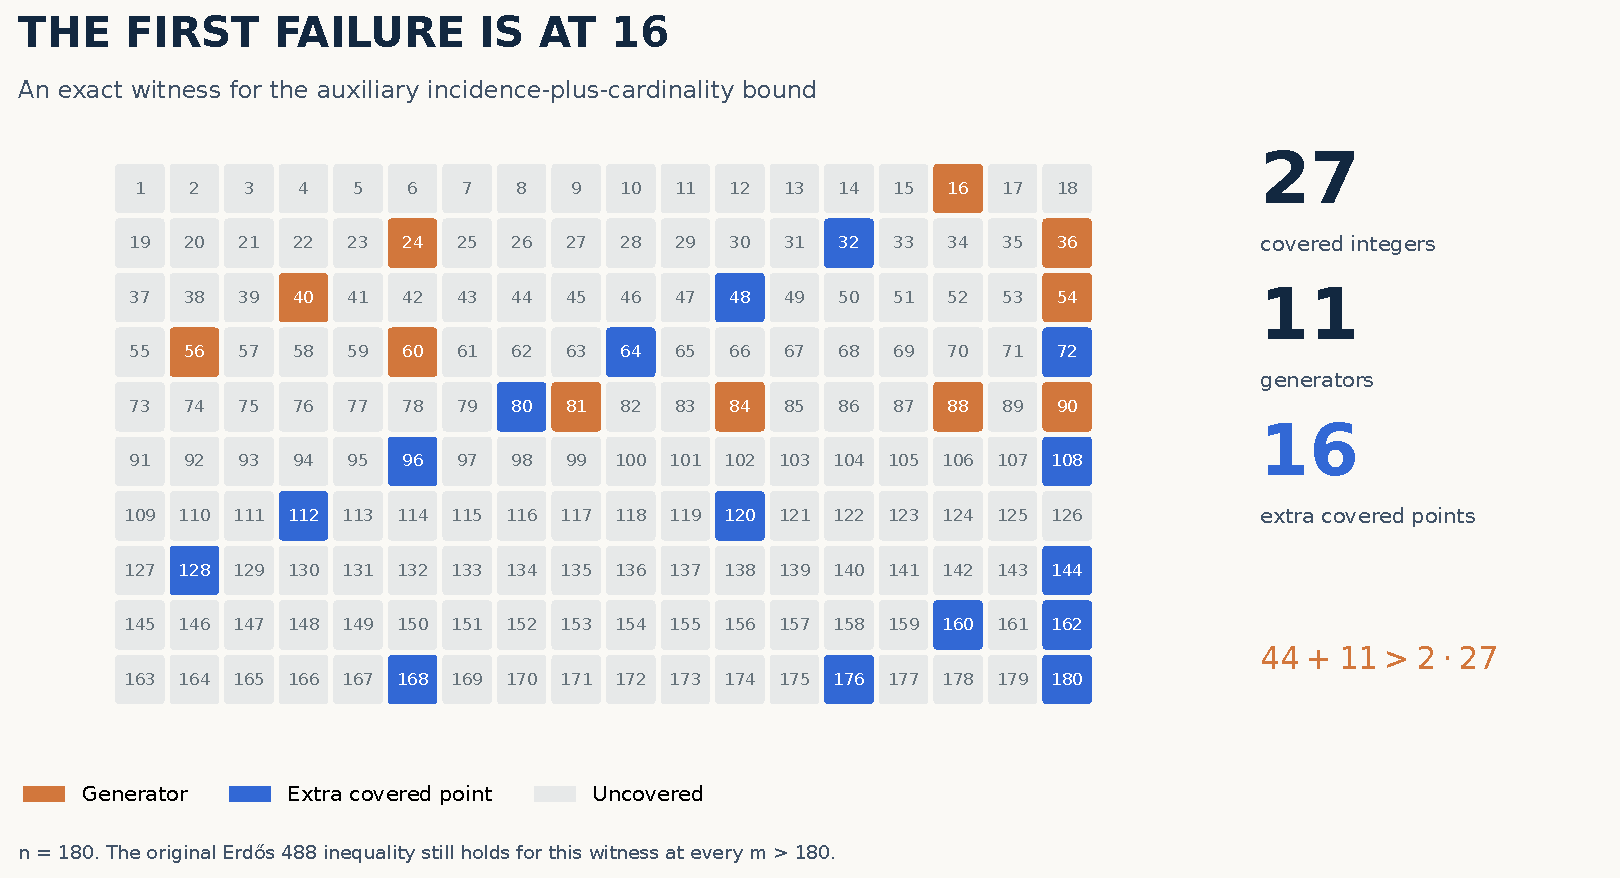
\includegraphics{figures/slack-barrier.pdf}
\caption{The first auxiliary failure at excess 16: orange generators and
blue extra covered points at n=180. The original Erd\texorpdfstring{\odoubleacute}{o}s 488 inequality
still holds for this witness for every m\textgreater180.}
\end{figure}

It is primitive and collectively coprime, \(54<180\), and \(55>54\).
Thus \(E=16\) and the auxiliary defect is exactly 1. Theorem 1 excludes
every smaller excess, establishing Theorem 2's first claim. The
corresponding Lean theorem states the minimum using \texttt{IsLeast}.

\hypertarget{the-sharp-family-at-arbitrary-sparsity}{%
\subsubsection{3.3. The sharp family at arbitrary
sparsity}\label{the-sharp-family-at-arbitrary-sparsity}}

For \(k\ge2\), put

\[
H_k=kG_0\cup\{180k-1\},\qquad n_k=180k. \tag{7}
\]

The map \(x\mapsto kx\) preserves the old covered and incidence counts.
The extra generator lies above \(n_k/2\), contributes only itself, and
is not divisible by \(k\). It is therefore new and uncovered by the old
generators. It neither divides nor is divided by an old generator.
Consequently,

\[
F_{H_k}(n_k)=28,\quad I_{H_k}(n_k)=45,\quad |H_k|=12.
\]

A common divisor of \(16k\) and \(81k\) divides \(k\); if it also
divides \(180k-1\), it is 1. This proves collective coprimality. Taking
\(k=R+M+2\) gives all inequalities in (3).

These examples do not refute (1). Indeed, exact rational arithmetic
gives

\[
180\sum_{g\in G_0}\frac1g<48,
\qquad
n_k\sum_{h\in H_k}\frac1h
=180\sum_{g\in G_0}\frac1g+\frac{180k}{180k-1}<50<56.
\]

Since \(56=2F_{H_k}(n_k)\), the rational union bound proves (1) for this
whole family and all \(m>0\). The number 16 is the sharp threshold for
\textbf{(2)} as a function of excess, not a threshold at which the
original conjecture is known to fail.

\hypertarget{why-the-excess-at-most-fifteen-proof-is-finite-and-complete}{%
\subsection{4. Why the excess-at-most-fifteen proof is finite and
complete}\label{why-the-excess-at-most-fifteen-proof-is-finite-and-complete}}

Put \(q_g=\lfloor n/g\rfloor\), and call \(g\) active when \(q_g\ge2\).
Its proper-multiple chain is

\[
C_g=\{2g,3g,\ldots,q_gg\}.
\]

Primitivity ensures that these points are not generators. Their union is
exactly \(B_G\cap[1,n]\setminus G\), of cardinality \(E\). Writing \(p\)
for the descending list of active quotients,

\[
W(p):=\sum_{q\in p}(q-1)=I_G(n)-|G|,
\]

the auxiliary estimate is equivalent to \(W(p)\le2E\).

Each active generator contributes a distinct doubled point, so there are
at most \(E\) active generators. Also \(q_g-1\le E\). The doubled
points, together with fourth and higher dyadic multiples where
applicable, give stronger capacity bounds: equality between distinct
dyadic multiples would make two generators divide one another. Distinct
generators with the same quotient have disjoint proper-multiple chains.
To see the latter, a common multiple has two distinct integer
coefficients at most that quotient; after reduction their ratio is too
far from 1 to allow both generators to have the same integer quotient.
The formal proof handles endpoint strictness explicitly.

Further restrictions come from exact pair-intersection capacities, ratio
uniqueness, and configurations of three or four quotient values. A
minimal auxiliary failure also gives deletion bounds and a connected
intersection pattern. These are proved implications about actual integer
families, rather than empirical filters.

For a connected family, divide generator coordinates by a chosen
smallest generator \(d\). A state contains rational pairs
\((r,q)=(g/d,\lfloor n/g\rfloor)\). Its endpoint interval is

\[
\max_{(r,q)} qr\ \le\ \frac nd\ <\ \min_{(r,q)}(q+1)r. \tag{8}
\]

If a new chain meets an existing proper-multiple point \(z\), its
coordinate must be \(z/j\) for some integer \(2\le j\le q\). This
produces finitely many successors. Each transition checks the quotient
budget, primitivity, interval feasibility, and the proper-point
capacity. A connected actual family has an ordering adding a chain that
meets the preceding union; the formal completeness theorem therefore
places it on a reachable path.

The certificates are finite tables of states with an initial-state
witness and checked successor coverage. A small-core
\texttt{NoCompletion} certificate proves that no reachable state can
realize all requested quotients. A full-profile \texttt{Safe}
certificate instead proves the needed auxiliary bound at every relevant
reachable state. The finite table is useful only after its local checks
and the generic reachability theorem have been combined.

For the final excess-15 layer, the complete construction includes 176
profile-enumeration blocks and 43 capacity blocks. Structural reductions
and 44 certified cores, containing 3,459 states in total, leave seven
profiles. Two final family graphs contain 6,263 states and 20,869 edges.
Their complete coverage and safety arguments are supplied to the final
theorem. These are counts of certificate states, not counts of distinct
integer families or of globally distinct states across all certificates.
Earlier excess layers are proved dependencies of the final result.

The search that suggests a profile or graph is outside the trust
boundary. The finite list's coverage, every needed edge, and the final
implication are checked in Lean. The definitions of \texttt{next},
\texttt{Bad}, and the original certificate semantics are not weakened to
obtain acceptance.

\hypertarget{pair-versus-tail-a-finite-refutation-and-an-unbounded-theorem}{%
\subsection{5. Pair-versus-tail: a finite refutation and an unbounded
theorem}\label{pair-versus-tail-a-finite-refutation-and-an-unbounded-theorem}}

\hypertarget{a-counterexample-with-all-generators-prime}{%
\subsubsection{5.1. A counterexample with all generators
prime}\label{a-counterexample-with-all-generators-prime}}

For \(a=2,b=3\), let \(V\) be the forty primes from 5 through 181. At
\(n=381,m=1468\), the kernel-checked counts are

\[
S_{2,3\mid V}(381)=29,\qquad S_{2,3\mid V}(1468)=224.
\]

Thus

\[
381\cdot224=85\,344>85\,144=2\cdot1468\cdot29.
\]

Every ordering and endpoint condition in Conjecture 4.8 of {[}2{]} is
met. All generators are distinct primes, so the example even has
pairwise coprimality. Below 381 the survivors are precisely the nonunit
numbers \(2^i3^j\), of which there are 29. Below 1468 there are 43 such
smooth numbers, together with \(2p,3p,4p,6p\), \(p>181\) prime,
contributing respectively 88, 51, 31, and 11 numbers. These categories
are disjoint.

\hypertarget{proof-of-theorem-3}{%
\subsubsection{5.2. Proof of Theorem 3}\label{proof-of-theorem-3}}

Choose a sufficiently large \(t\), set \(n=2^{2t}\), and let \(V\)
consist of all primes \(p\) with \(b<p\le n\). Take \(t\) large enough
that \(n>M\) and \(V\ne\varnothing\). Every survivor below \(n\) has all
prime factors at most \(b\). Its prime-exponent vector injects into a
finite set with at most

\[
(2t+1)^{b+1}
\]

elements. Therefore \(S_{a,b\mid V}(n)\le(2t+1)^{b+1}\), while \(a\)
itself ensures this count is positive.

Let \(Q=\prod_{p\in V}p\). An elementary comparison with the product
over consecutive odd integers yields

\[
Q\le2^{t+1}\varphi(Q). \tag{9}
\]

For example, the proved Euler-product estimate is
\(1\le4n(\varphi(Q)/Q)^2\), which implies (9). This estimate requires no
prime number theorem.

Set \(m=a(n+1)Q\). For each of \(n+1\) complete residue blocks, the
multiples of \(a\) indexed by residues coprime to \(Q\) survive the
tail. Hence

\[
S_{a,b\mid V}(m)\ge(n+1)\varphi(Q).
\]

Combining the two count bounds gives

\[
\frac{nS_{a,b\mid V}(m)}{mS_{a,b\mid V}(n)}
\ge\frac{2^{t-1}}{a(2t+1)^{b+1}}.
\]

A proved elementary exponential-versus-polynomial lemma lets us choose
\(t\) with \(2aK(2t+1)^{b+1}<2^t\). This proves (4). Since every tail
prime exceeds \(b\), and \(a\nmid b\), the combined generator set is
primitive.

\hypertarget{sparse-amplification-and-incidence-growth}{%
\subsection{6. Sparse amplification and incidence
growth}\label{sparse-amplification-and-incidence-growth}}

\hypertarget{separated-copies}{%
\subsubsection{6.1. Separated copies}\label{separated-copies}}

Let \(G_0\subseteq[2,n_0]\) be primitive. For \(L\ge1\) and \(N>n_0L\),
define

\[
G_{L,N}=\bigcup_{0\le i<L}(N+i)G_0,
\qquad n_*=n_0(N+L).
\]

For each \(i<L\), \(\lfloor n_* /(N+i)\rfloor=n_0\). Moreover, the map

\[
(i,u)\longmapsto(N+i)u,\qquad 0\le i<L,\quad1\le u\le n_0,
\]

is injective. Indeed, distinct \(u,v\) would force a gap of at least
\(N\) to be compensated by a term smaller than \(n_0L\). Thus the
covered sets of the copies are disjoint, and

\[
F_{G_{L,N}}(n_*)=LF_{G_0}(n_0),\quad
I_{G_{L,N}}(n_*)=LI_{G_0}(n_0),\quad |G_{L,N}|=L|G_0|. \tag{10}
\]

The same separation argument proves primitivity across copies. Applying
(10) to (6) yields the exact defect \(L\). If \(L\ge2\), two consecutive
scales together with the base elements 16 and 81 force collective gcd
one. Increasing \(N\) provides arbitrary sparsity and an arbitrary
lower-endpoint threshold.

\hypertarget{proof-of-theorem-4}{%
\subsubsection{6.2. Proof of Theorem 4}\label{proof-of-theorem-4}}

The divergence of the sum of reciprocals of primes is classical and is
imported from Mathlib {[}3{]}. Choose a finite prime set \(P\),
containing 2 and 3, with reciprocal sum sufficiently large, and put

\[
N_0=2\prod_{p\in P}p.
\]

All selected primes divide \(N_0\), so there is an exact identity

\[
I_P(N_0)=N_0\sum_{p\in P}\frac1p.
\]

The formal finite-selection argument makes \(I_P(N_0)>K(N_0+1)\), in
particular \(I_P(N_0)>KN_0\ge KF_P(N_0)\). Apply the separated-copies
construction with two adjacent scales. Equation (10) preserves the
strict incidence inequality. The base primes 2 and 3 and the adjacent
scales ensure collective gcd one. Choosing the scale sufficiently large
also gives both sparse inequalities and \(M<n\).

Bare unboundedness of \(I/F\) is already an immediate consequence of
prime-reciprocal divergence and \(F_P(N_0)\le N_0\). The formal result
recorded here includes the simultaneous restrictions in (5); no novelty
is claimed for the classical divergence theorem or for that elementary
unrestricted consequence.

\hypertarget{formal-verification-and-reproducibility}{%
\subsection{7. Formal verification and
reproducibility}\label{formal-verification-and-reproducibility}}

The accepted sources use Lean 4.33.1 and Mathlib at commit
\texttt{0df444a360\allowbreak{}eaa60ab8c1\allowbreak{}1dca51a86a\allowbreak{}f692955474} {[}3,4{]}. Accepted
module checks were run with trust level zero (\texttt{-t\ 0}); large
computations also use a single Lean worker (\texttt{-j\ 1}). The
reported dependencies are only the standard logical axioms
\texttt{propext}, \texttt{Classical.\allowbreak{}choice}, and \texttt{Quot.\allowbreak{}sound}.
The delivered proofs use no \texttt{sorry}, \texttt{admit},
\texttt{native\_\allowbreak{}decide}, or project-specific axioms.

\begin{longtable}[]{@{}
  >{\raggedright\arraybackslash}p{(\columnwidth - 2\tabcolsep) * \real{0.5000}}
  >{\raggedright\arraybackslash}p{(\columnwidth - 2\tabcolsep) * \real{0.5000}}@{}}
\toprule\noalign{}
\begin{minipage}[b]{\linewidth}\raggedright
Mathematical result
\end{minipage} & \begin{minipage}[b]{\linewidth}\raggedright
Principal Lean source and declaration
\end{minipage} \\
\midrule\noalign{}
\endhead
\bottomrule\noalign{}
\endlastfoot
Theorem 1, auxiliary estimate & \texttt{ExcessFifteenMain.\allowbreak{}lean}:
\texttt{ExcessFifteen.\allowbreak{}excess\_\allowbreak{}at\_\allowbreak{}most\_\allowbreak{}fifteen\_\allowbreak{}union\_\allowbreak{}bound} \\
Theorem 1, original inequality & \texttt{ExcessFifteenMain.\allowbreak{}lean}:
\texttt{ExcessFifteen.\allowbreak{}erdos488\_\allowbreak{}excess\_\allowbreak{}at\_\allowbreak{}most\_\allowbreak{}fifteen} \\
Reduction of a general input set & \texttt{PrimitiveCoreBounds.\allowbreak{}lean}:
\texttt{erdos488\_\allowbreak{}core\_\allowbreak{}excess\_\allowbreak{}at\_\allowbreak{}most\_\allowbreak{}fifteen} \\
Explicit sparse slack refutations & \texttt{ProofsCore.\allowbreak{}lean},
\texttt{Proofs.\allowbreak{}lean}, \texttt{SmallSlack.\allowbreak{}lean} \\
Least failure excess & \texttt{SharpSlackThreshold.\allowbreak{}lean}:
\texttt{sixteen\_\allowbreak{}is\_\allowbreak{}least\_\allowbreak{}failure\_\allowbreak{}excess} \\
Sharp sparse coprime family & \texttt{SharpSparseThreshold.\allowbreak{}lean}:
\texttt{arbitrarily\_\allowbreak{}sparse\_\allowbreak{}coprime\_\allowbreak{}sharp\_\allowbreak{}failure} \\
Least excess with all restrictions & \texttt{SharpSparseLeast.\allowbreak{}lean}:
\texttt{sixteen\_\allowbreak{}is\_\allowbreak{}least\_\allowbreak{}sparse\_\allowbreak{}coprime\_\allowbreak{}failure} \\
The sharp family satisfies the original inequality &
\texttt{SharpSparseOriginal.\allowbreak{}lean}:
\texttt{sharp\_\allowbreak{}sparse\_\allowbreak{}family\_\allowbreak{}original} \\
Finite pair-tail refutation & \texttt{ProofsSmall.\allowbreak{}lean} \\
Theorem 3 & \texttt{GeneralPairTail.\allowbreak{}lean}:
\texttt{every\_\allowbreak{}primitive\_\allowbreak{}pair\_\allowbreak{}has\_\allowbreak{}unbounded\_\allowbreak{}tail\_\allowbreak{}density\_\allowbreak{}ratios} \\
Exact additive defect & \texttt{UnboundedSlackDefect.\allowbreak{}lean}:
\texttt{arbitrary\_\allowbreak{}sparse\_\allowbreak{}coprime\_\allowbreak{}exact\_\allowbreak{}defect} \\
Theorem 4 & \texttt{UnboundedSlackRatio.\allowbreak{}lean}:
\texttt{arbitrary\_\allowbreak{}sparse\_\allowbreak{}coprime\_\allowbreak{}incidence\_\allowbreak{}ratio} \\
\end{longtable}

Files are rooted at \texttt{research/\allowbreak{}} in the accompanying project.
\texttt{research/\allowbreak{}REPRODUCE.\allowbreak{}md} and \texttt{research/\allowbreak{}verify\_\allowbreak{}bundle.\allowbreak{}py}
give the import-ordered source rebuild. The source archive's manifest
fixes the inputs; verification records retain actual exit codes and
hashes. Checking a final module against compiled imports is
distinguished from rebuilding all imported sources. Selected final
entrypoints also have independent agent rebuilds and semantic audits;
this does not mean every audit rebuilt the entire dependency graph.

The workspace required a startup adapter because procfs was unavailable.
It supplies the known executable path and calls the original Lean
entrypoint; it does not modify proof checking. The original executable
and shared-library hashes were compared with the official release. A
conventional Linux installation uses the official release without this
adapter.

Memory-terminated, interrupted, and superseded attempts are not accepted
proofs. They are retained separately from successful checks. Finite
certificates are accepted only after their exact statements and relevant
imports have actually compiled successfully.

\hypertarget{related-work-provenance-and-the-role-of-computation}{%
\subsection{8. Related work, provenance, and the role of
computation}\label{related-work-provenance-and-the-role-of-computation}}

The problem statement is pinned to a versioned formal-conjectures source
{[}1{]}, consulted as a specification and never imported as an assumed
open theorem. Chojecki's manuscript {[}2{]} proves an
excess-at-most-five theorem and proposes the two auxiliary conjectures
refuted here. Our references to its numbering mean the PDF dated 20
March 2026, with SHA-256

\begin{Shaded}
\begin{Highlighting}[]
\NormalTok{68639a31a69302089202a71b156425cf5db6f08e7f43fc91ed1869faaeecf5a3}
\end{Highlighting}
\end{Shaded}

The same manuscript's Proposition 7.2 already constructs a prime-tail
example for a singleton head with density ratio exactly 2. Prime-tail
screening therefore has an explicit precursor; it is not claimed as a
newly invented idea. The strict counterexamples and the quantified
fixed-pair extension are separate statements. Likewise, the standard
union bound, elementary scaling, prime-reciprocal divergence, and the
integer sequence containing (6) are not claimed as discoveries of this
project.

Targeted prior-art checks did not establish global priority. In
particular, a relevant August 2026 discussion could not be fully
inspected; indexed fragments are not a substitute for its proof or
attachments. The defensible claim is that the displayed statements were
derived and formally checked in this project, and that Theorem 1
improves the explicit excess range in the inspected March manuscript.
Whether all strengthened formulations are new across the literature
remains open to external assessment.

The research also included an original-problem counterexample search
with 21,600.003879 seconds of recorded effective wall time. Pauses were
excluded; parallel CPU time was not substituted for elapsed time. No
counterexample was found in the tested inputs. This is a search record,
not evidence for an unbounded exclusion theorem. A separate \(N=25\)
branch of Erd\texorpdfstring{\odoubleacute}{o}s problem 686 obtained formal boundary lemmas and finite
negative searches, but contributes no theorem to the present paper.

OpenAI Codex agents generated conjectural approaches, search programs,
candidate certificates, Lean proof text, mathematical explanations, and
this manuscript. Separate agents reviewed several proof interfaces and
rebuilt selected entrypoints. Such agent review is not external peer
review. The human user set the research objective and authorized
publication; no human author identity or institutional endorsement is
inferred. Mathematical trust rests on the explicit statements and
successful kernel checks, subject to the usual trust in the
proof-assistant implementation and its stated logical foundations.
Exposition, priority claims, and software packaging still require human
scrutiny.

\hypertarget{beyond-the-auxiliary-threshold-a-pending-extension}{%
\subsection{9. Beyond the auxiliary threshold: a pending
extension}\label{beyond-the-auxiliary-threshold-a-pending-extension}}

\textbf{Status at preparation: the complete excess-at-most-sixteen
theorem is not yet claimed.} The failure of (2) at excess 16 does not
prevent a proof of (1) using a sharper bound. For a normalized state
\(s\) with upper endpoint \(u(s)\), reciprocal sum \(R(s)\), and
covered-point count \(U(s)\),

\[
u(s)R(s)\le2U(s)
\]

is sufficient: the actual normalized endpoint is strictly smaller than
\(u(s)\). For a nonempty partial state, a separately proved rule bounds
the missing reciprocal contribution using the remaining quotients. It
explicitly retains the actual equality \(F_G(n)=|G|+16\); it is not an
unproved monotonicity claim about numerically promising prefixes.

A complete 626-state certificate already proves the original inequality
for the specific active quotient profile \([11,7,5,4,3,3,3,2,2,2,2]\),
under \(E\le16\), without ambient connectedness or activity assumptions.
The broader program has certified five shared graphs covering sixteen
remaining profiles and the selected core exclusions. The full raw
capacity coverage needed to connect that finite list to every actual
input is still pending at this manuscript's preparation. Consequently,
none of those components is substituted here for a completed general
E≤16 theorem.

\hypertarget{appendix-a.-the-initial-instruction-and-the-actual-interaction}{%
\subsection{Appendix A. The initial instruction and the actual
interaction}\label{appendix-a.-the-initial-instruction-and-the-actual-interaction}}

The original user instruction is reproduced verbatim below, including
its mixed Chinese and English wording. It was a broad research
objective, not a supplied mathematical construction or proof.

\begin{quote}
我有个有趣的主意，首先，你来梳理近代以来数学界所有low hanging
fruit，找到20个可用lean解决的问题，但未被AI和人类解决的问题，然后找到问题以后作出可行性分析，在此基础上对一个相对最容易解决的问题发起攻关，允许你使用agent，允许使用一切工具，允许使用lean进行形式化验证，允许使用一切最新资料进行佐证，该问题需具备数学上的开创意义，能够有效推进人类的认知边界，你的结果必须要经过lean的验证，禁止作弊，禁止修改规则，禁止说解决不出来放弃，至少尝试6h。你可以使用multi
agent，全自主编排，现在开始，至少运行六个小时，给你完整授权，你可以安装所有你需要的软件，运算资源使用无上限
\end{quote}

\textbf{English translation.}

\begin{quote}
I have an interesting idea. First, survey all the low-hanging fruit in
mathematics since modern times and find 20 problems that can be solved
using Lean but have not been solved by AI or humans. After identifying
the problems, analyze their feasibility and, on that basis, launch an
attack on one that is relatively the easiest to solve. You may use
agents, all tools, Lean for formal verification, and all the latest
materials as supporting evidence. The problem must have pioneering
mathematical significance and effectively advance the boundary of human
knowledge. Your results must pass Lean verification. No cheating, no
changing the rules, and no saying that you cannot solve it and giving
up. Try for at least 6 hours. You may use multiple agents with fully
autonomous orchestration. Start now and run for at least six hours. You
have my full authorization. You may install all the software you need,
and there is no upper limit on computational resources.
\end{quote}

The agents selected Erd\texorpdfstring{\odoubleacute}{o}s 488 from the candidate review, designed the
constructions and search programs, and developed the Lean proofs. The
interaction did not end with this initial instruction: the user later
asked the agents to resume after token-limit interruptions and
subsequently authorized preparation of a public GitHub project and
publication materials. The workflow therefore should not be described as
an uninterrupted, one-click solution. Its recorded search duration is
cumulative effective runtime, as explained above.

The instruction's requested scope and ambition are not themselves claims
achieved by the paper. In particular, this work supplies a bounded
candidate survey, conditional original-problem theorems, and auxiliary
counterexamples and strengthenings; it does not establish a complete
catalogue of modern open mathematics or solve the unrestricted Erd\texorpdfstring{\odoubleacute}{o}s 488
problem. The mathematical literature, Lean, and Mathlib remain
explicitly credited.

\hypertarget{references}{%
\subsection{References}\label{references}}

\begin{enumerate}\raggedright
\def\labelenumi{\arabic{enumi}.}
\tightlist
\item
  The Formal Conjectures Authors. \emph{Erd\texorpdfstring{\odoubleacute}{o}s Problem 488}. Versioned
  formal statement, commit
  \texttt{8323e878b8\allowbreak{}3fcd7f4a44\allowbreak{}8256069352\allowbreak{}a265460d75}.
  \href{https://github.com/google-deepmind/formal-conjectures/blob/8323e878b83fcd7f4a448256069352a265460d75/FormalConjectures/ErdosProblems/488.lean}{Primary
  source}.
\item
  Przemyslaw Chojecki. \emph{Signed Transport, Pair--Tail Reduction, and
  Low Layers in an Erd\texorpdfstring{\odoubleacute}{o}s Density-Doubling Problem}. Manuscript dated 20
  March 2026; inspected version identified by the hash above.
  \href{https://www.ulam.ai/research/erdos488.pdf}{Primary manuscript}.
\item
  The Mathlib Community. \emph{Mathlib}, commit
  \texttt{0df444a360\allowbreak{}eaa60ab8c1\allowbreak{}1dca51a86a\allowbreak{}f692955474}; in particular
  \texttt{Mathlib/\allowbreak{}NumberTheory/\allowbreak{}Sum\allowbreak{}Prime\allowbreak{}Reciprocals.\allowbreak{}lean}.
  \href{https://github.com/leanprover-community/mathlib4/blob/0df444a360eaa60ab8c11dca51a86af692955474/Mathlib/NumberTheory/SumPrimeReciprocals.lean}{Pinned
  primary source}.
\item
  The Lean Project. \emph{Lean 4}, release v4.33.1.
  \href{https://github.com/leanprover/lean4/releases/tag/v4.33.1}{Official
  release}.
\end{enumerate}

The accompanying \texttt{refs.\allowbreak{}bib} supplies these references in BibTeX
format. The bibliography records sources used for problem provenance and
established ingredients, not an assertion of a complete literature
survey.

\end{document}
